% template:x02 GDC:YES
\begin{question}
  \hspace*{\fill} [Note Maximale: ?]\par
  \medskip
  \noindent Indroduction à la question.\par
  \medskip
  \begin{center} % or flushleft or flushright
    \noindent Commentaire au-dessus du diagramme\par
    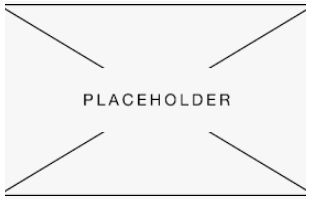
\includegraphics[scale=0.3]{placeholder}\par
    \noindent Commentaire en-dessous du diagramme\par
  \end{center} % or flushleft or flushright

  % Option 2. A question broken down into a list of parts each with its component maximum mark
  \noindent Peut-être quelques elements generals de la question - elements auquels les parties de la question peuvent se reférer - suivis ensuite d'úne question en parties.\par
  \begin{enumerate}[label=(\alph*)]
    \item une partie de la question\hspace*{\fill} [?]
    \item une autre partie sub-divisé
      \begin{enumerate}[label=(\roman*)]
        \item une sub-division de la partie %\hspace*{\fill} [?]
        \item une autre sub-division\hspace*{\fill} [?]
      \end{enumerate}
    \item une derniére partie\hspace*{\fill} [?]
  \end{enumerate}
\end{question}
